\section{Post-processing \& Results}

One of the benefits of using a FEM software like COMSOL is its advanced post-processing capabilities.
This allows the user to examine the physics driving VI in great detail.
Figure \ref{fig:model_pressure} shows the resulting pressure field from solving Darcy's Law, as well as the associated airflow streamlines in the soil.
Here we see the pressure in the near foundation crack region is roughly the same as the house pressurization of \SI{-5}{\pascal}, which quickly decreases towards the ground surface.
It is also apparent how this pressure field induces a airflow from the ground surface, with air near the house heading relatively straight to the foundation crack, whereas the air further away from the house penetrates deeper into the soil and almost "whirlwinds" underneath the house.\par

\begin{figure}[htb!]
  \centering
  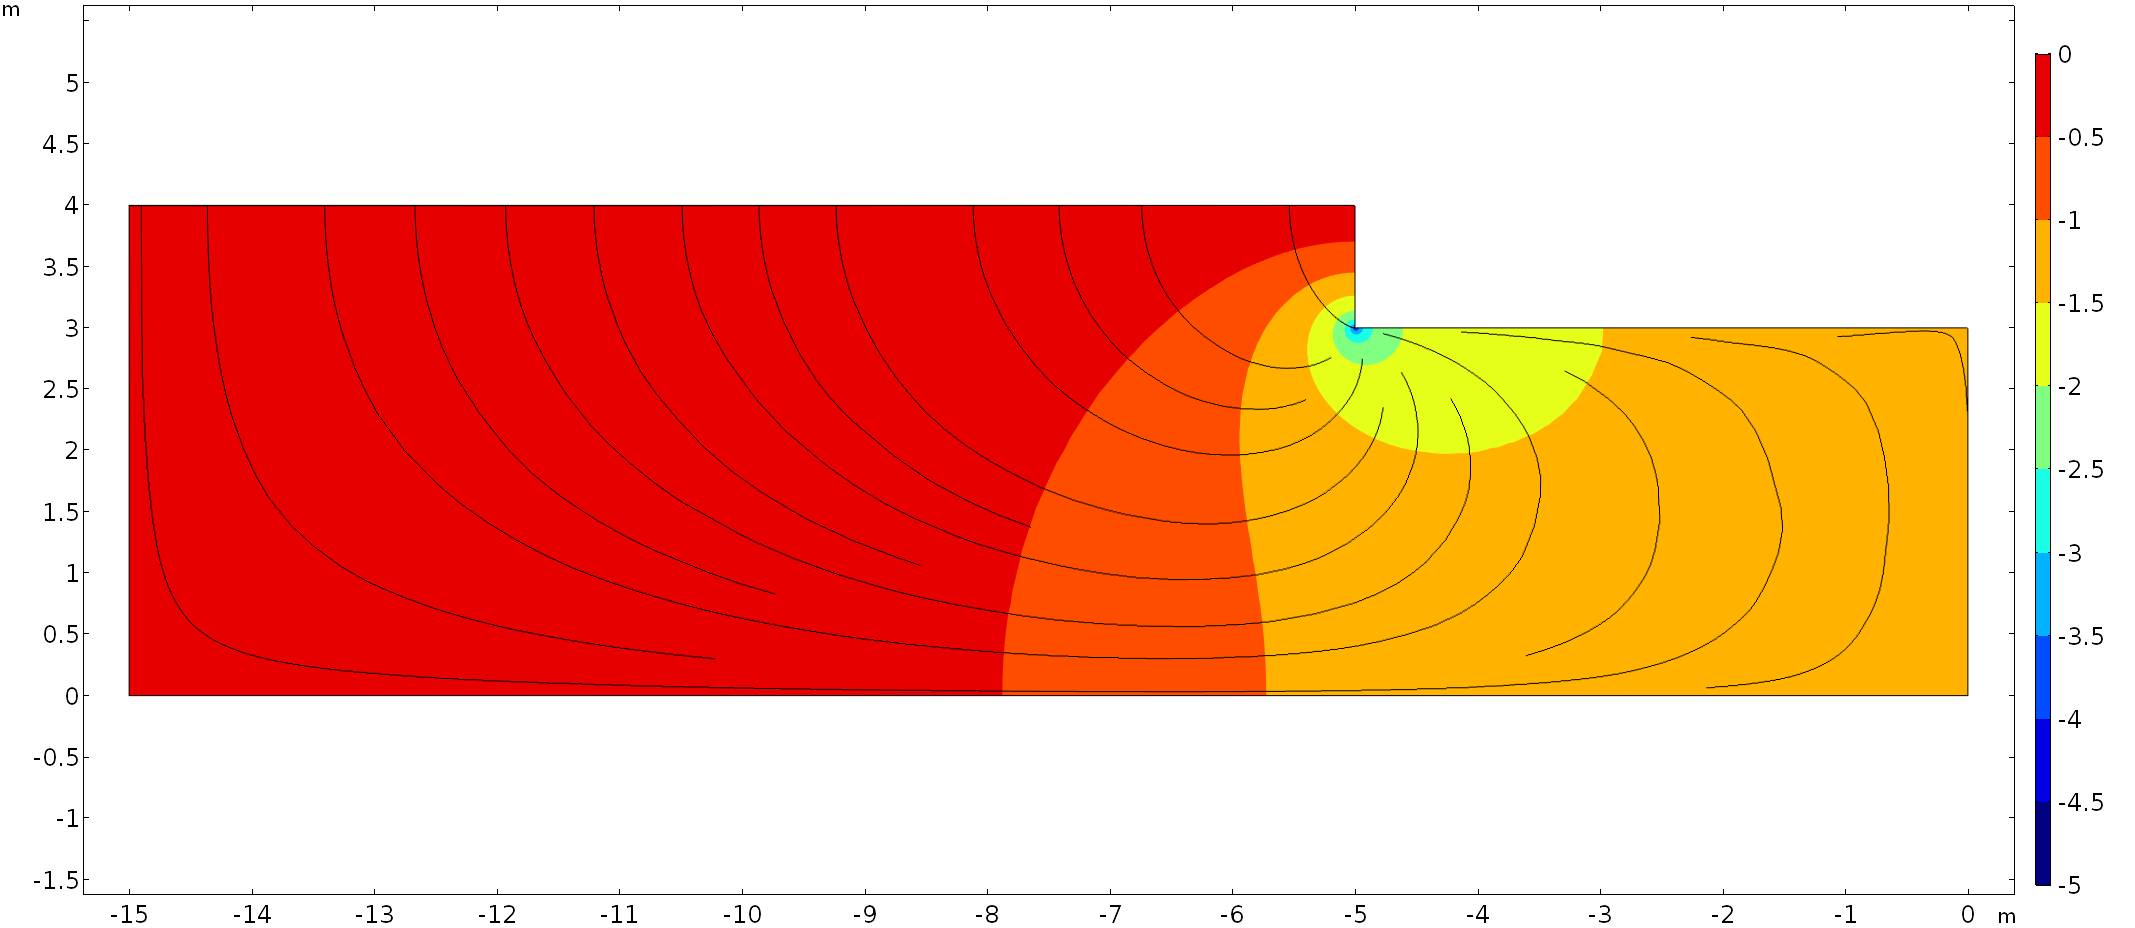
\includegraphics[width=0.75\textwidth]{model_pressure.png}
  \caption[Modeled Darcy's pressure field in soil]{Pressure field from Darcy's Law with associated airflow streamlines.}
  \label{fig:model_pressure}
\end{figure}

\begin{figure}[htb!]
  \centering
  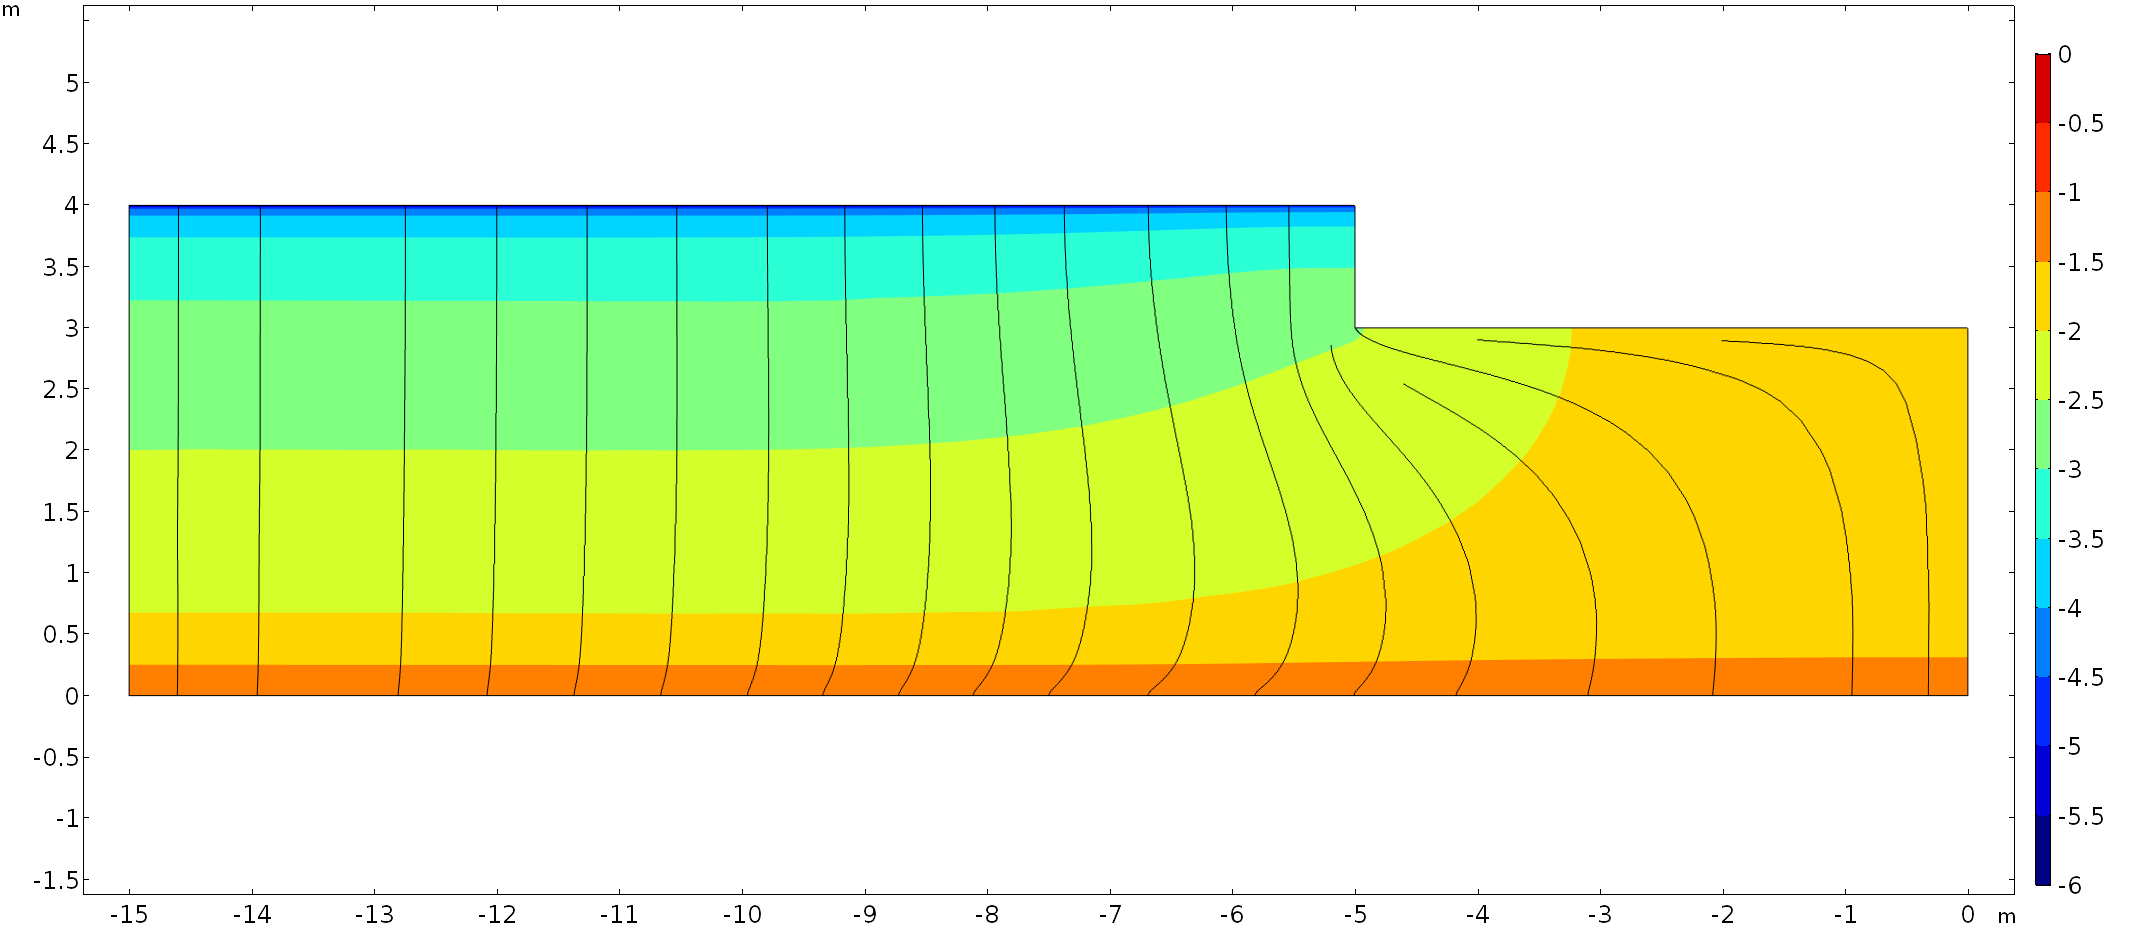
\includegraphics[width=0.75\textwidth]{model_concentration.png}
  \caption[Modeled contaminant concentration in soil]{Contaminant concentration in the soil, normalized to groundwater concentration and log-transformed, with transport streamlines.}
  \label{fig:model_concentration}
\end{figure}

The contaminant concentration in the soil, normalized to the groundwater source concentration and log-transformed, with the contaminant flux streamlines, is examined in Figure \ref{fig:model_concentration}.
Here see that far away from the house, the contaminant vapor simply diffuse straight from the groundwater source to the atmosphere, while beneath the house foundation, contaminant vapors accumulate because the foundation acts as a diffusion blocker.
Based on those streamlines we can conclude that the advective component of the flux is very here small.
Perhaps surprisingly, we do not see a significant advective transport downwards along the wall of the house.
However, considering that the soil type is sandy loam, airflow velocities are expected to be small.\par

One might think that advective transport is large in the horizontal direction along the foundation slab, as the transport and airflow streamlines are so similar.
However, by inspecting Figure \ref{fig:model_velocity_crack} we see that airflow velocities are not greater here than elsewhere, and therefore the advective transport is not either.
To make sense of this, we can inspect the horizontal diffusive flux, divided by the magnitude of the total flux
\begin{equation}
  \frac{j_\mathrm{diff,y-direction}}{|j_\mathrm{total}|}
\end{equation}
to see what portion of the total contaminant flux transport the diffusive horizontal represents here.
Figure \ref{fig:model_horizontal_diff} shows that the horizontal contaminant transport underneath the foundation is in fact driven by the large contaminant concentration gradient between the region underneath and outside the house foundation.
This shows the power of modeling and how it can reveal things that at first seem intuitively correct, but in fact are not.\par

\begin{figure}[htb!]
  \centering
  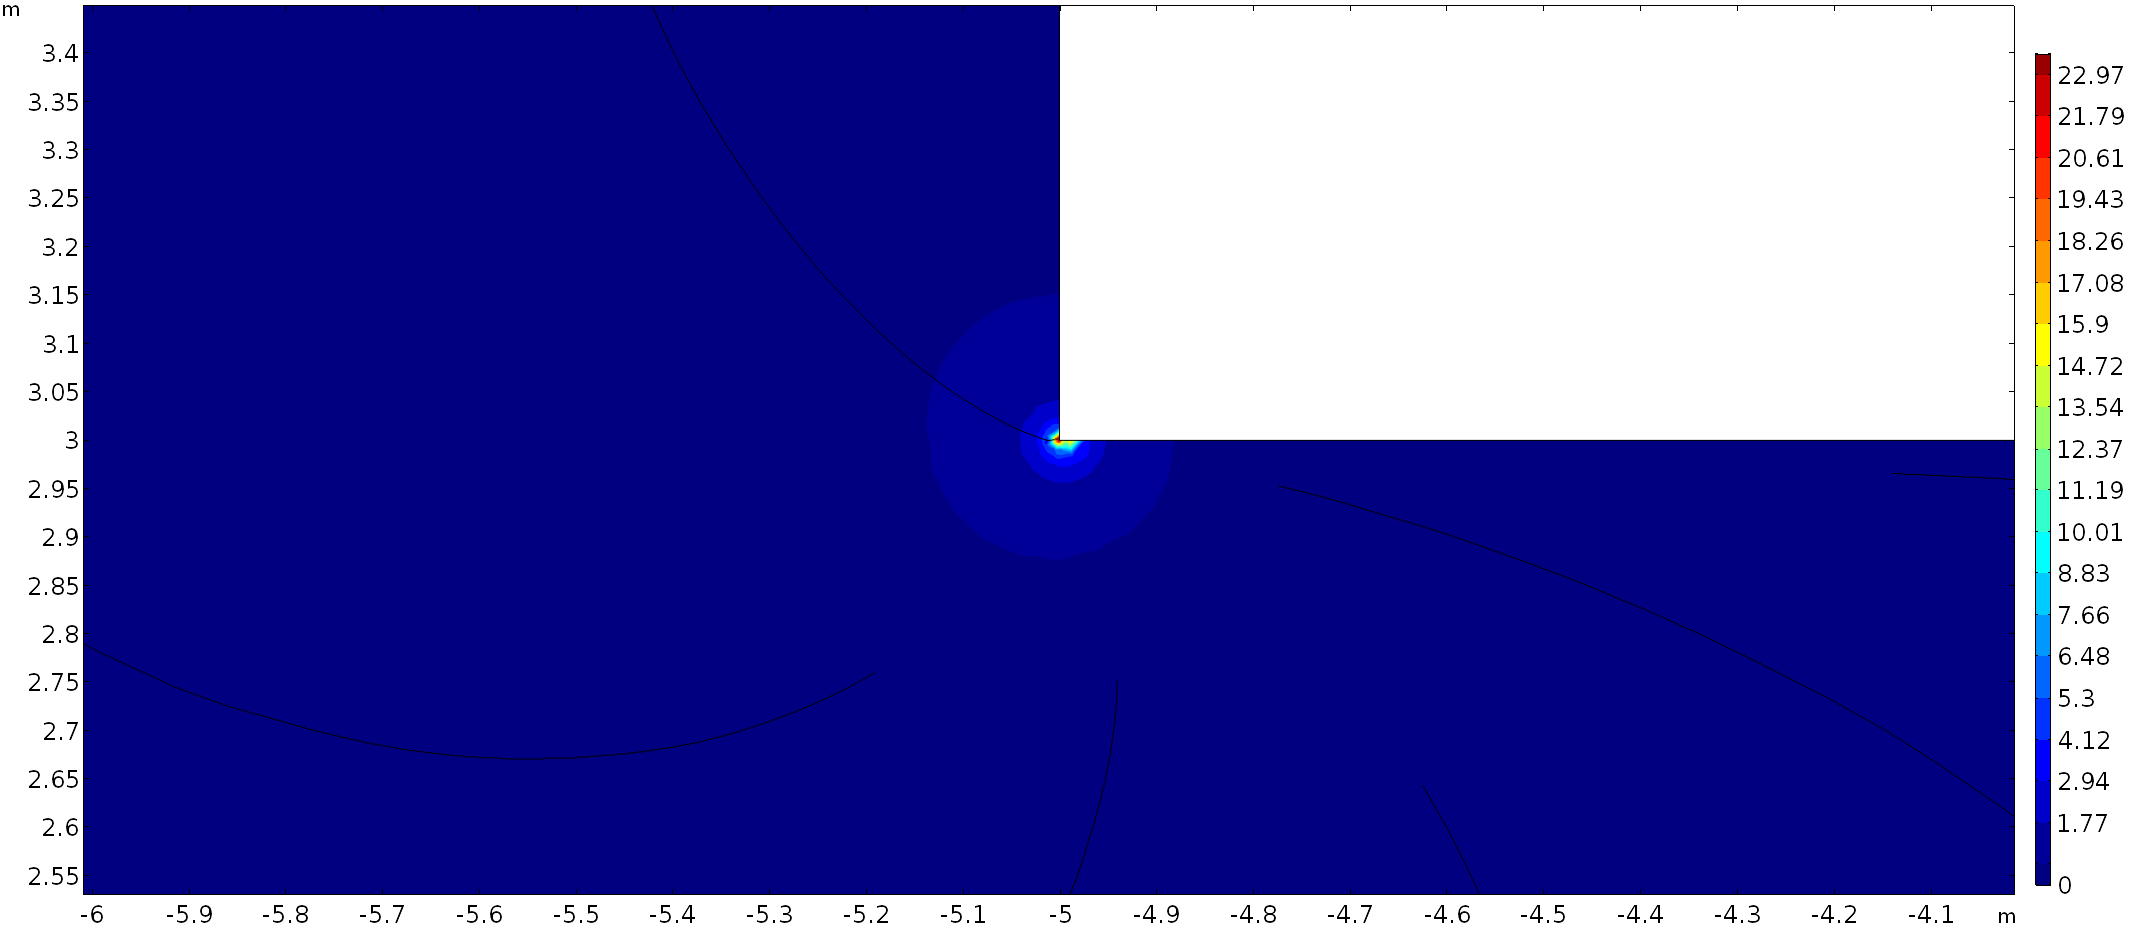
\includegraphics[width=0.75\textwidth]{model_velocity_crack.png}
  \caption{Airflow velocity $\vec{u}_g$ [\si{\milli\metre\per\hour}] near the foundation crack with associated its streamlines.}
  \label{fig:model_velocity_crack}
\end{figure}

\begin{figure}[htb!]
  \centering
  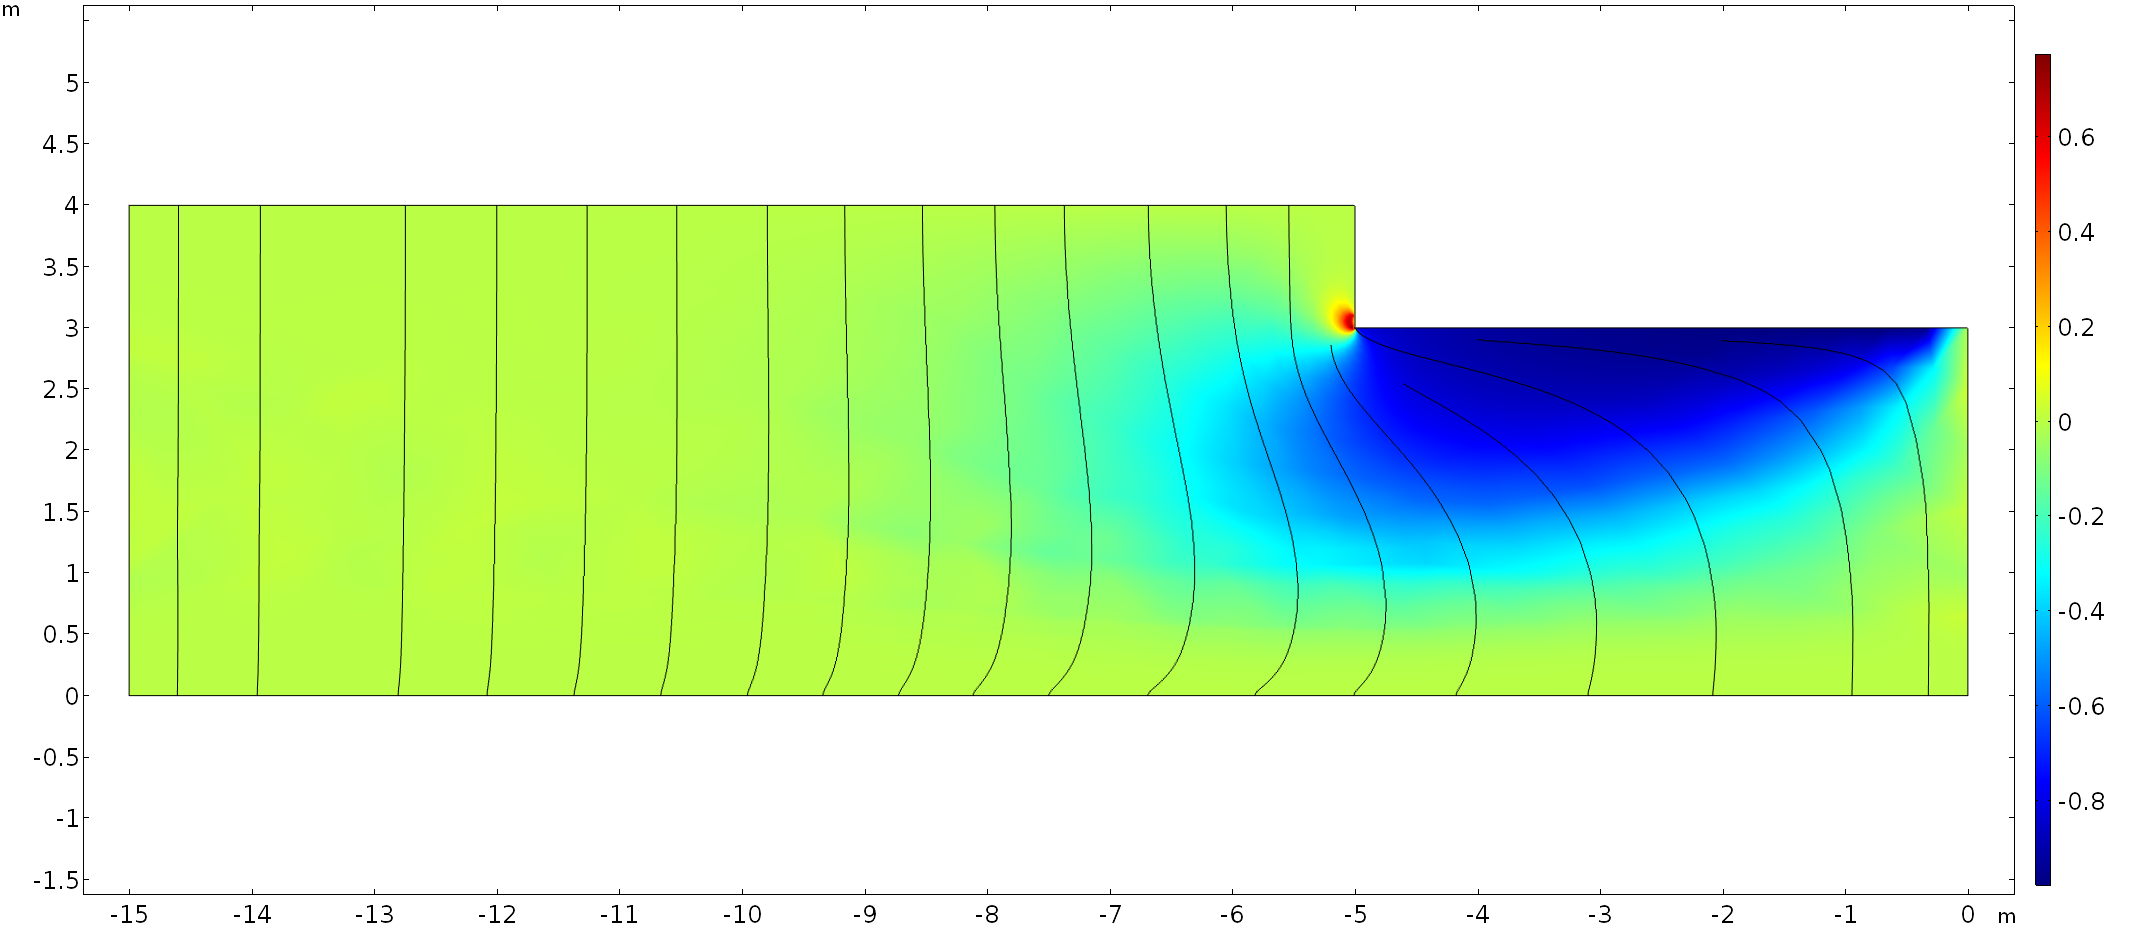
\includegraphics[width=0.75\textwidth]{model_transport_flux_y.png}
  \caption[Analysis of horizontal diffusion flux.]{Horizontal (y-axis) diffusive flux component normalized to the magnitude of the total flux. A value of 1 here indicates that the total contaminant transport flux is due to diffusion, while 0 would indicate the opposite - that all contaminant transport is due to advection. The sign signifies the direction, with positive and negative values indicating a flux in the rightward and leftward direction respectively. E.g. a value of -0.8 indicates that the 80\% of the magnitude of the contaminant transport is due to horizontal (along the y-axis) diffusion, and occurs leftward.}
  \label{fig:model_horizontal_diff}
\end{figure}

Another useful feature of post-processing is that it can be used for bug searching and to evaluate where the mesh can be potentially improved.
When the transport equation is used to numerically model contaminant transport, there is a tendency for the solution to oscillate around the "true" solution, and thereby violate mass conservation, if the mesh size in a particular element is too large.
This can be quantified by the cell Péclet number, which characterizes the relative magnitude of advection/diffusion in a cell.
\begin{equation}
  \mathrm{Pe_{cell}} = \frac{\mathrm{adv_{cell}}}{\mathrm{diff_{cell}}} = \frac{u_g h}{2 D_\mathrm{eff}}
\end{equation}
here $u_g$ [\si{\metre\per\second}] is the soil-gas airflow velocity;
$h$ [\si{\metre}] is the mesh size in the element or cell;
and $D_\mathrm{eff}$ [\si{\metre\squared\per\second}] is the effective diffusivity in the cell.
If $\mathrm{Pe_{cell}} > 1$ there is a risk that this oscillating behavior will manifest.
Small exceedances, $~\mathrm{Pe_{cell}} < 25$, are usually mitigated by various stabilization schemes, which are inherently integrated into COMSOL as well as many other FEM packages, but for larger values further mesh refinement may be required.\par

Figure \ref{fig:model_cell_peclet} shows $\mathrm{Pe_{cell}}$ as a volume plot, and excludes all values that fall below one.
As we can see, only the region close to the groundwater exceeds $\mathrm{Pe_{cell}}$, which is due to the very small $D_\mathrm{eff}$ there.
The exceedance is small, so the stabilization scheme is able to compensate which is confirmed by Figure \ref{fig:model_concentration} (no oscillations visible).
This is also a region where even if such oscillations occurred, would probably not affect the indoor contaminant concentration.
Regardless, Figure \ref{fig:model_cell_peclet} shows where the mesh may potentially be refined, which comes in handy to know if one runs a model where airflow velocities are significantly higher than in this example.\par

\begin{figure}[htb!]
  \centering
  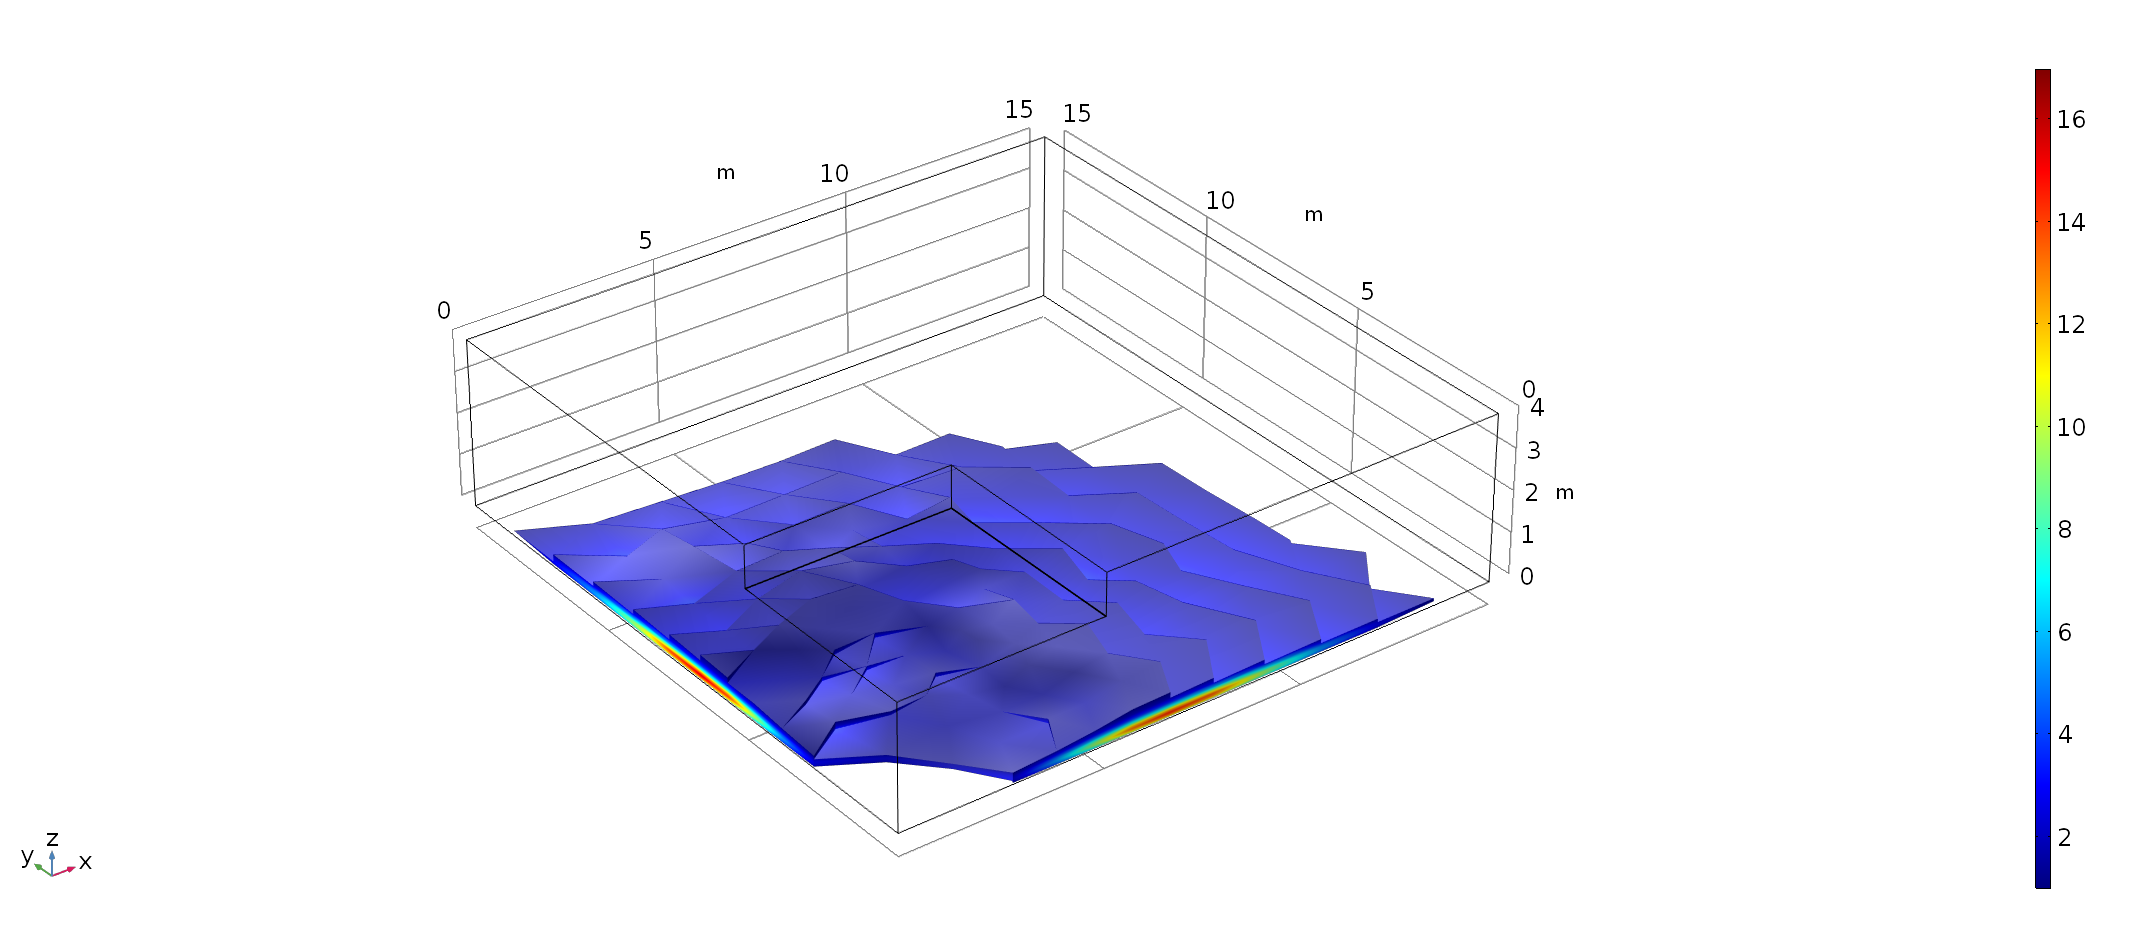
\includegraphics[width=0.75\textwidth]{model_cell_peclet.png}
  \caption{Volume plot showing where the cell Péclet number exceeds 1 and its actual value. I.e. it suggests where the mesh may be improved.}
  \label{fig:model_cell_peclet}
\end{figure}
